\documentclass[10pt]{article}

\usepackage{cite}
\usepackage{lipsum}
\usepackage{url}
\usepackage{float}
\usepackage{amsmath}
\usepackage{enumitem}
\usepackage{graphicx}
\usepackage{caption}
\usepackage{subcaption}
\usepackage{rotating}
\usepackage{geometry}
\usepackage{listings}
\usepackage{hyperref}
\usepackage[T1]{fontenc}
\usepackage[numbered]{matlab-prettifier}
\usepackage{mathtools}


\newcommand{\documentTitle}{CAAM 564 Project: Optimization Algorithms for Support Vector Machines}
\newcommand{\documentAuthors}{Wei Wu}
\newcommand{\reportDate}{May 1, 2019}

\geometry{margin=1in}
\lstset{
	tabsize=4,
	basicstyle={\ttfamily},
	captionpos=b,
	belowskip=1em,
	aboveskip=1em,
	numbers=left,
	escapechar=\@,
}

\title{
	\textbf{\documentTitle}
}
\author{\textit{\documentAuthors}}
\date{\textit{\today}}

\setlength{\parindent}{0pt}
\setlength{\parskip}{1em}


\begin{document}
	%%%% Write an abstract if needed
	%\begin{abstract}
	%You can add an abstract at the beginning of the article.
	%\end{abstract}
\maketitle
	
\section{Introduction} 

The support vector machines (SVMs) are popular supervised machine learning models, first introduced in (Boser, Guyon and Vapnik 1992 \cite{boser1992training}, Cortes and Vapnik 1995 \cite{cortes1995support}). SVMs have since gained attention in the machine learning community and have been applied widely to classification problems such as text/spam classification \cite{joachims1998text} \cite{tong2001support}. In this project, however, we take an under-the-hood exploration of the SVMs: we are primarily interested in the mathematical formulation of the model, and the numerical solution to its underlying quadratic programming problem. This project is partially inspired by my experience with one of the homework of COMP 540 Statistical Machine Learning at Rice University.  

\section{Mathematical Formulation}
\subsection{Hard Margin SVMs}

The classic hard margin SVMs are usually posed in the following form

\begin{equation}\label{eq:1}
\begin{aligned}
& \underset{w,b}{\text{minimize}}
& & \frac{1}{2} \lVert w \rVert_{2}^2 
& \text{subject to}
& & y_i(\langle w,x_i \rangle - b) \geq 1, \; i = 1, \ldots, n.
\end{aligned}
\end{equation}

where each data point $(x_i,y_i)$ consists of features vector $x_i \in R^m$ and class labels $y_i$. In this project, we consider the two-class support vector machines, and hence $y_i \in \{-1, +1\}$. 

Rewrite the inequality constraints as 
\begin{equation}
	g_i(w) = -y_i(\langle w,x_i\rangle - b) + 1 \leq 0.
\end{equation}

The hard margin SVM forms a quadratic programming problem, with its Lagrangian
\begin{equation}
	L(w,b,\alpha) = \frac{1}{2} \lVert w \rVert_{2}^2 + \sum_{i=1}^{n}\alpha_i(1 - y_i(\langle w,x_i \rangle - b)). 
\end{equation} 

The primal and dual solutions satisfy the Karush-Kuhn-Tucker (KKT) conditions. In particular, we have the following
\begin{subequations}\label{eq:4}
\begin{align}
0 = \nabla_{w} L(w,b,\alpha) = w - \sum_{i}^{n}\alpha_i y_i x_i \label{eq:4a}\\
0 = \frac{\partial}{\partial b} L(w,b,\alpha) = \sum_{i}^{n}\alpha_i  \label{eq:4b}
\end{align}
\end{subequations}

With the above identities, we yield the following expression of the dual function:
\begin{equation}
\begin{aligned}
q(\alpha) 
& = \underset{w,b}{\text{min}}\: L(w,b,\alpha)\\
& = \frac{1}{2} \Bigg \lVert \sum_{i}^{}\alpha_i y_i x_i \Bigg \rVert_{2}^2  + \sum_{i}^{}\alpha_i (1-y_i \Bigg \langle \sum_{j}^{}\alpha_j y_j x_j,x_i \Bigg \rangle + y_i b )\\
& = \frac{1}{2} \sum_{i,j}^{}\alpha_i \alpha_j y_i y_j \langle x_i, x_j\rangle - \sum_{i,j}^{}\alpha_i \alpha_j y_i y_j \langle x_i, x_j\rangle + \sum_{i}^{}\alpha_i(y_i b + 1)\\
& = \sum_{i}^{}\alpha_i - \frac{1}{2} \sum_{i,j}^{}\alpha_i \alpha_j y_i y_j \langle x_i, x_j\rangle
\end{aligned}
\end{equation}
 

This leads to our dual optimization problem $\underset{\alpha \geq 0}{\text{max}} \: \underset{w,b}{\text{min}}\: L(w,b,\alpha)$ with the following form
\begin{equation} \label{eq:6}
\begin{aligned}
& \underset{\alpha}{\text{max }} 
\sum_{i}^{}\alpha_i - \frac{1}{2} \sum_{i,j}^{}\alpha_i \alpha_j y_i y_j \langle x_i, x_j\rangle
\text{ subject to }
\alpha \geq 0, \text{ and }
\sum_{i}^{} \alpha_i y_i = 0.
\end{aligned}
\end{equation}

Note that from the KKT conditions, we also get $\alpha_i > 0 $ only for data points where the corresponding inequality constraints holds with equality, i.e. $g_i(w) = 0$. These $x_i$'s are called the support vectors. The solution $(w^*, b^*)$ to \eqref{eq:1} gives an halfspace defined by $\langle w, x\rangle + b = 0$, which serves as the separating hyperplane (a decision boundary) to classify data points. If we add one more feature to each features vector, we can elimiate the bias term $b = 0$. In this case, the support vectors are at distance $1/||w^*||$ to the separating hyperplane, and in fact span $w^*$, a result by applying the Fritz-John (or Karush-John) optimality conditions \cite{Shalev-Shwartz:2014:UML:2621980}, or simply from \eqref{eq:4a} :

\begin{center}
	\textit{Let $I = \{i: |\langle w^*, x_i\rangle| = 1\}$. Then there exists coefficients $\alpha_1,...,\alpha_n$ such that $w^*  = \sum_{i \in I}^{}\alpha_i x_i$}
\end{center}

\subsection{Soft Margin SVM}
The hard-margin SVM does not have a solution if the data is not linearly separable. Further, even if the data is linearly separable, the solution is highly sensitive to outliers. To address this, we add a slack variable $\xi$ and relax the hard inequality constraint, but penalize large violations:

\begin{equation}\label{eq:1}
\begin{aligned}
& \underset{w,b}{\text{minimize}}
& & \frac{1}{2} \lVert w \rVert_{2}^2 + C \sum_{i=1}^{n}\xi_i
& \text{subject to}
& & y_i(\langle w,x_i \rangle - b) \geq 1 - \xi_i,
& & \xi_i \geq 0, \; i = 1, \ldots, n.
\end{aligned}
\end{equation} 

Note that $C \geq 0$ is a hyperparameter to the model that regularizes the penalty of large slack variable.  

The soft margin SVM in its primal form is equivalent to the following unconstrained optimization problem

\begin{equation}\label{eq:8}
\begin{aligned}
& \underset{w,b}{\text{minimize}}
& & \frac{1}{2} \lVert w \rVert_{2}^2 + C \sum_{i=1}^{n}max(1 - y_i(\langle w, x_i\rangle-b), 0)
\end{aligned}
\end{equation} 


The dual form of the soft margin SVM could be found in a similar way where we obtain the dual form of the hard margin SVM. I omit the derivation and simply present the result below

\begin{equation} \label{eq:9}
\begin{aligned}
& \underset{\alpha}{\text{max }} 
\sum_{i}^{}\alpha_i - \frac{1}{2} \sum_{i,j}^{}\alpha_i \alpha_j y_i y_j \langle x_i, x_j\rangle
\text{ subject to }
0 \leq \alpha \leq C, \text{ and }
\sum_{i}^{} \alpha_i y_i = 0.
\end{aligned}
\end{equation}


\subsection{Usage of Kernel}
The equations \eqref{eq:6} and \eqref{eq:9} alludes to the usage of kernel trick. If we apply a feature mapping $\psi$ to each of the feature vector $x$, then we obtain a kernel function $K(x,x') = \langle \psi(x), \psi(x')\rangle$. By applying the feature mapping, and therefore the kernel function, we embed the input space into some high dimensional feature space, and hence enable our SVM to learn nonlinear decision boundary in the input space. Whether a kernel function is valid is governed by the Mercer's theorem, which states a kernel function is valid if its associated kernel matrix is positive-semidefinite.

Some common kernel functions include the class of linear kernels $K(x,y) = x^T y + b$ and the class of Gaussian kernels $K(x,y) = exp(- \frac{||x - y||^2}{2\sigma})$. From now on we assume a kernelized version of soft margin SVMs.

\section{Optimization Algorithms}
This primal formulation \eqref{eq:8} gives rise to a simple stochastic (sub)gradient descent (SGD) algorithm for the soft margin SVM (e.g. \cite{shalev2007online}), since it fits exactly within the framework of solving regularized loss minimization problem with SGD. Other algorithms focused on solving the primal form were also proposed (e.g. \cite{chapelle2007training}). 

The numerical solution to the dual form \eqref{eq:9} is more extensively, especially studied during the early 2000s. Some active sets algorithms are proposed in \cite{scheinberg2006efficient} and \cite{vogt2005active}. Both algorithms are much more complexed than the SGD-based algorithm. Another popular and simpler numerical algorithm to solve the dual form is the so-called Sequential Minimal Optimization, first proposed in \cite{platt1998sequential}, and its implementation \textit{libsvm} \cite{CC01a} remains one of the SVM implementations (SVC) of the scikit-learn library \cite{scikit-learn}. One rudimentary implementation of SMO could be found here \cite{svm_smo_impl}  

For this project, I implemented an SGD-based SVM, and also an SMO-based SVM by modifying a solver found online. From the practical perspective, one difference between the two algorithms is that the SGD-based SVM does not compute support vectors on the fly, while the SMO-based SVM gives the support vectors naturally by solving the dual problem. The support vectors could potentially be used by a machine learning practitioner to interpret the model. 

The code for both implementations could be found in the \href{https://github.com/wwJinkla/SVM}{Github repository} for this project. The file \textit{SMO.py} contains the implementations of the SMO-based model. The files \textit{linear\textunderscore svm.py} and \textit{linear\textunderscore classifier.py} contain the implementation of the SGD-based model. Both implementations uses helper functions from \textit{utils.py}. The IPython notebook \textit{SVM.ipynb} contains demo code of both models. Some visualization results on small synthetic datasets could be found on the next page. Note that the decision boundaries are subject to hyperparameters tunning.       
\pagebreak

\newpage

\begin{figure}
	\centering
	\begin{subfigure}{.5\textwidth}
		\centering
		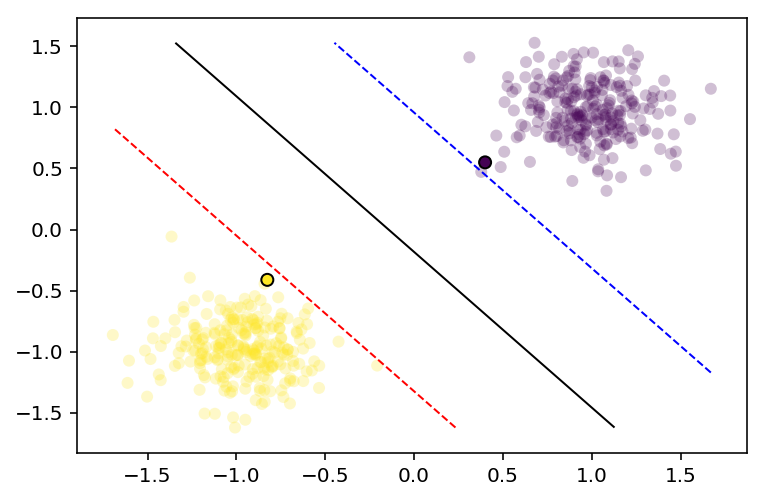
\includegraphics[width=\linewidth]{fig1}
		\caption{SMO result with decision boundary + support vectors (highlighted)}
		\label{fig:linearSMO}
	\end{subfigure}%
	\begin{subfigure}{.5\textwidth}
		\centering
		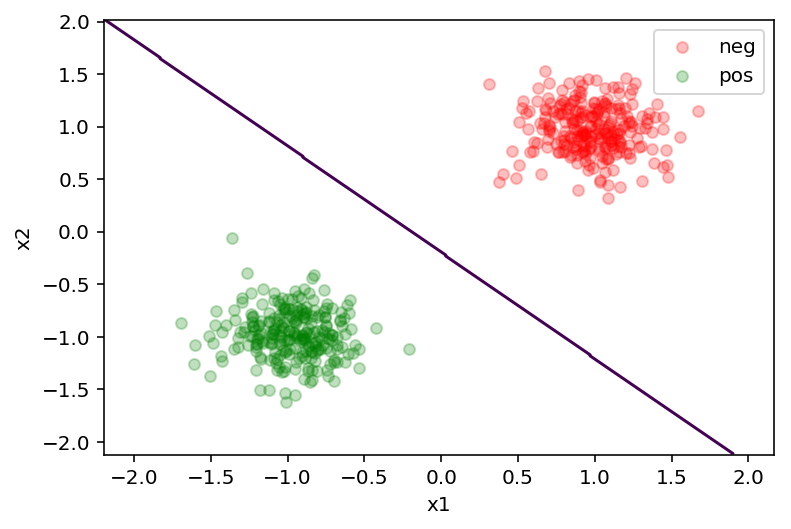
\includegraphics[width=\linewidth]{fig2}
		\caption{SGD result with decision boundary}
		\label{fig:linearSGD}
	\end{subfigure}
	\caption{Linearly Separable Data}
	\label{fig:test}
\end{figure}


\begin{figure}
	\centering
	\begin{subfigure}{.5\textwidth}
		\centering
		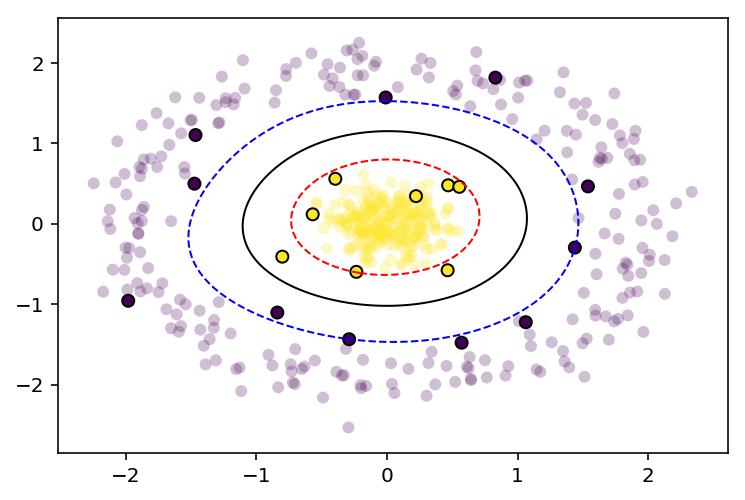
\includegraphics[width=\linewidth]{fig3}
		\caption{SMO result with decision boundary + support vectors (highlighted)}
		\label{fig:nonlinearSMO}
	\end{subfigure}%
	\begin{subfigure}{.5\textwidth}
		\centering
		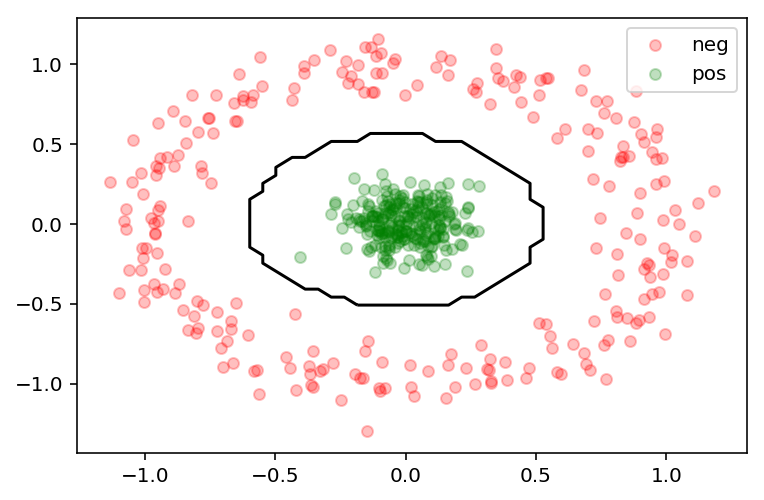
\includegraphics[width=\linewidth]{fig4}
		\caption{SGD result with decision boundary}
		\label{fig:nonlinearSGD}
	\end{subfigure}
	\caption{Non-Linearly Separable Data}
	\label{fig:test}
\end{figure}

\pagebreak
\clearpage

\newpage
\section{Conclusion/Reflection}
In this project, we examined the mathematical formulation of Support Vector Machines, and implemented two of the commonly used algorithms to solve the underlying optimization problem. 

Originally I wished to implement the active sets method presented in \cite{scheinberg2006efficient} to further my understanding of the active sets method learned in CAAM 564, but it turned out to be too ambitious. A more thorough examination of and an own implementation of the SMO algorithm is left as my future work.    

\clearpage
\bibliography{reportBib}{}
\bibliographystyle{plain}

	
\end{document}